% Chapter Template

\chapter{Proposed Work} % Main chapter title

\label{ch:proposed} % Change X to a consecutive number; for referencing this chapter elsewhere, use \ref{ChapterX}

\lhead{Chapter 5. \emph{Proposed}} % Change X to a consecutive number; this is for the header on each page - perhaps a shortened title

Given the results in Chapter \ref{ch:results}, we consider the proposed work to complete as part of completing
degree work.

%----------------------------------------------------------------------------------------
%	SECTION 1
%----------------------------------------------------------------------------------------
\section{Adaptive Sparse Grid}

We have demonstrated in a preliminary manner the effectiveness of a method proposed by \cite{Gerstner} and used in
\cite{Ayres} where the polynomial index set to be
used in constructing the sparse grid quadrature is constructed adaptively.
%effectiveness in a preliminary manner in this work, but 
We observed opportunity for further improvements critical
in exploring this method's potential.  The algorithm proceeds generally
as follows:
\begin{itemize}
  \item Begin with the mean (zeroth-order) polynomial expansion.
  \item While not converged:
    \begin{itemize}
      \item Collect a list of the polynomial index set whose predecessors have all been evaluated.
      \item Predict the impact of adding each polynomial to the existing polynomial index set.
      \item If the total impact of all indices is less than tolerance, convergence is reached.
      \item Otherwise, add the predicted highest-impact polynomial and loop back.
    \end{itemize}
\end{itemize}
This adaptive algorithm has the strength of determining the appropriate anisotropy to apply when generating a
polynomial index set.  For anisotropic cases, or cases where the static index set construction rules are not
ideal, the adaptive index set could potentially provide a method to avoid wasted calculations and emphasize
high-impact polynomials in the expansion.  Fig. \ref{fig:asg_step} shows an example process for a
two-dimensional input space. In this example, the axis represent orders of included polynomials, the blue
squares indicate index set polynomials already included, and the green circle indicates the next most
impactful candidate for inclusion.  In this example, it is evident polynomials in $y_1$ have an overall
greater impact on the response variance than $y_1$.

\begin{figure}[H]
  \centering
  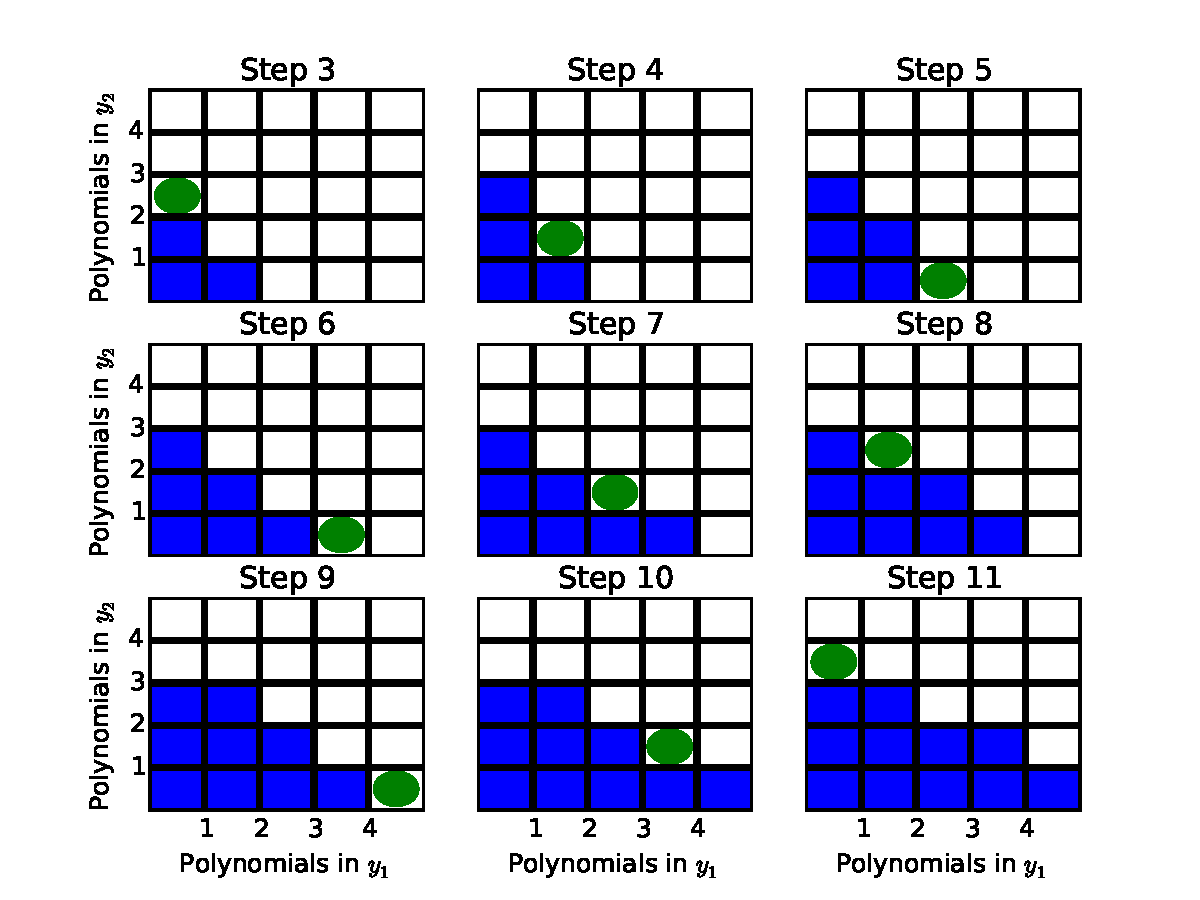
\includegraphics[width=0.9\linewidth]{asc_block}
  \rule{35em}{0.5pt}
  \caption{Adaptive Sparse Grid Steps}
  \label{fig:asg_step}
\end{figure}

There are, however, some weak points in this algorithm.  First, the algorithm in literature has no predictive method
to determine the next polynomial index to include in the set; instead, it evaluates each potential index and
selects the one with the most impact \cite{Ayres}.  This is somewhat inefficient, because of SCgPC representations created
that are not used in the final product.  In addition to including this algorithm, we propose to develop a
method for predicting high-impact points based on the impact of their predecessors in the set.  Results shown
in this work are a first step in that direction.

Second, there are certain types of models for which the adaptive algorithm will stall or converge too early.
For instance, if the partial derivative of the model with respect to any of the
input dimensions is zero when evaluated at the mean point (but nonzero elsewhere), the algorithm will falsely
converge prematurely, as adding additional polynomial orders to the input in question will not change the
value of the model at the mean point.  For example, consider a model
\begin{equation}
  f(a,b) = a^3b^3,
\end{equation}
with both $a$ and $b$ uniformly distributed on [-1,1].  We note the partial derivatives with respect to either
input variable evaluated at the central point (0,0) are zero.  The first polynomial index set point to
evaluate is zeroth-order in each dimension, [0,0].  We distinguish input domain points from polynomial index
set points by using parenthesis for the former and square brackets for the latter. The quadrature point to
evaluate this polynomial coefficient is (0,0), which, when evaluated, gives $f(0,0)=0$.  The next polynomial
index set combinations are [1,2] and [2,1].  For [1,2], the quadrature points required are
(0,$\pm\sqrt{1/3}$).  This evaluates to $f(0,\pm\sqrt{1/3})=0$, as well.  Because of symmetry, we obtain the
same result of [2,1].  According to our algorithm, because our old value was 0, and the sum of the new
contributions is 0, we have converged; however, we know this is false convergence.  While we expect few
applications for SCgPC to exhibit these zero partial derivatives in the input space, it is a limitation to be
aware of.  In addition to implementing this algorithm, we propose to find a way either to work around this
limitation, or at least to warn the user when such a case is likely to exist.


\section{Adaptive HDMR}
Despite the benefits of ideal anisotropic polynomial set construction promised by the adaptive SCgPC
algorithm, we expect the adaptive SCgPC to fall short for models where many input parameters provide relevant
uncertainty.  While the adaptive polynomial index set construction can preferentially emphasize particular
dimensions, it does not reduce the input cardinality of the problem.  An additional algorithm presented in
\cite{Ayres} uses an adaptively-constructed HDMR representation to alleviate the curse of dimensionality for
the adaptive SCgPC method.

In the HDMR expansion, subsets of the input domain can be
joined together to approximate the full model,
\begin{align}
  u(Y) = u_0 &+ \sum_{n=1}^N u_{Y_n} \nonumber\\
  &+ \sum_{n_1=1}^N \sum_{n_2=1}^{n_1-1} u_{Y_{n_1},Y_{n_2}} \nonumber \\
  &+ \sum_{n_1=1}^N \sum_{n_2=1}^{n_1-1} \sum_{n_3=1}^{n_2-1} u_{Y_{n_1},Y_{n_2},Y_{n_3}} \nonumber \\
  &\cdots \nonumber\\
  &+u_{Y_{n_1},\cdots,Y_{n_N}},
\end{align}
where $u(Y)$ is the model, $Y$ is the combined input space, and $u_{Y_n}$ is an SCgPC surrogate model where
only $Y_n$ is considered varying and other input parameters are held at their reference value.  In static
HDMR, the desired largest subset size is selected, and all subset combinations are considered.  For instance,
for a model $f(a,b,c)$, the full HDMR expansion is
\begin{align}
  f(a,b,c,d) = f_0 &+ f_a + f_b + f_c \label{eq:exhdmr1}\\
    &+ f_{ab} + f_{ac} + f+{bc} \label{eq:exhdmr2}\\
    &+ f_{abc}. \label{eq:exhdmr3}
\end{align}
Truncating, a first-order HDMR expansion includes just the terms in Eq.\ref{eq:exhdmr1}, and a second-order
expansion additionally includes all the terms in Eq.\ref{eq:exhdmr2}.  However, it is entirely possible and
often likely that
some subsets have larger impact than others, and some might be ignored altogether without significantly
impacting the overall expansion.  Adaptive HDMR (AHDMR) is an algorithm that considers the potential impacts
of adding new polynomials to existing subsets (as in the Adpative Sparse Grid algorithm) as well as the
potential impact of adding new subsets to the HDMR expansion. The AHDMR algorithm proceeds as follows:
\begin{itemize}
  \item Evaluate the reference (all mean) case.
  \item Construct all first-order expansion surrogate models.
  \item While not converged:
  \begin{itemize}
    \item Using existing subset sensitivities, predict the importance of future subsets
    \item Consider the impact of adding polynomial indices to existing subset PCE representations
    \item Choose between expanding existing subsets or adding new subsets based on impact
    \item If the relative contribution of the new HDMR expectation is less than tolerance, convergence is
      reached.
  \end{itemize}
\end{itemize}
All the surrogate models for each subtype in the expansion are constructed using adaptive SCgPC expansions.
Because the input space for the subset surrogates is small, and grows slowly as the method progresses, they
are ideally suited for SCgPC methods.  However, we note that any surrogate model, or the original model
itself, can be used instead of adaptive SCgPC reduced-order models.

For the case demonstrated by \cite{Ayres}, combining adaptive HDMR and adaptive SCgPC makes it possible to
compete in convergence with Monte Carlo for input spaces with cardinality nearly up to a thousand.  Adding
more efficient polynomial index set choices for adaptive SCgPC, we expect to see additional increases in 
performance.

\section{Quadrature}
The numerical integrations in this work have all been performed using classic Gaussian quadrature sets
(Legendre, Hermite, Laguerre, Jacobi).  It is also possible to use other quadrature sets for integration, such
as Clenshaw-Curtis or Gauss-Patterson.  These quadratures have the benefit of nested quadratures when chosen
correctly, which, especially for adaptive methods, can save considerable computation.  We propose to implement
at least one of these nested quadratures and contrast the performance of SCgPC methods using both classic and
nested quadratures.

\section{Engineering Application}
Lastly, we propose to implement all of the methods discussed here in production-scale uncertainty
quantification code \raven{}, and apply them in quantifying the uncertainty of a nonlinear multiphysics
problem.  In particular, we propose considering a two-dimensional quarter-pin cell nuclear engineering problem
coupling \moose{} applications \rattlesnake{}, a neutron transport code, and \bison{}, a fuel performance
code.
